\documentclass[11pt,A5]{article}
\usepackage[utf8]{inputenc}
\usepackage[spanish]{babel}
\usepackage[rmargin=2.5cm,lmargin=3cm,tmargin=3cm,bottom=3cm]{geometry}

\usepackage{fancyhdr}
    \pagestyle{fancy}
        \fancyhf{}
        \rhead{\textcolor{white}{\thepage}}
        \cfoot{\textcolor{white}{Jordán Aarón Duarte Martínez}}
        \lhead{\textcolor{white}{\textsc{CUANDO SE CREA CON ALMA Y CORAZÓN}}}

\usepackage[x11names]{xcolor}
    \definecolor{doradu_mamalun}{RGB}{241,196,15}
    \definecolor{doradu_semimamalun}{RGB}{158,132,26}
    \definecolor{rosa_neon}{RGB}{255,0,239}
    \definecolor{rojo_violaceo_apagado}{RGB}{240,34,115}
    \definecolor{morado_neon}{RGB}{164, 59, 255}
    \definecolor{azul_triste}{RGB}{80,135,198}
    \definecolor{cafe_esperanza}{RGB}{224,132,15}
    \definecolor{beige_anaranjado}{RGB}{234,169,60}
    \definecolor{rojo_violaceo_luminoso}{RGB}{255,77,147}
    \definecolor{aguamarina}{RGB}{50,229,178}
    \definecolor{gris}{RGB}{96,96,100}
    \definecolor{azul_palido}{RGB}{160,247,255}
    \definecolor{doradu_opacu}{RGB}{127,105,19}
    \definecolor{beige_anaranjado_claro}{RGB}{255,184,67}
    \definecolor{verde_podredumbre}{RGB}{7,121,12}
    \definecolor{naranja_calido_luminoso}{RGB}{255,168,0}
    \definecolor{moradu}{RGB}{73,46,145}

\usepackage{graphicx}
\usepackage{caption}
\usepackage[rightcaption]{sidecap}
\parindent=0mm


\begin{document}
\pagecolor{black}
\color{white}

%Abajo se encuentra el título para nada improvisado sin usar "\maketitle" Bv.

\begin{center}
    {\textcolor{doradu_mamalun}{\textbf{\textsc{\underline{\Huge{A R C A N E}}}}}}
\end{center}

\begin{center}
    {\textcolor{doradu_mamalun}{\textbf{\textsc{\large{La serie Maestra del futuro}}}}}
\end{center}

\begin{center}
    {\textcolor{doradu_semimamalun}{\textsc{Por Jordán Aarón Duarte Martínez}}}
\end{center}

\section*{\Large{\textsf{\hspace{1.8cm}CUANDO SE CREA CON ALMA Y CORAZÓN}}}

Muchas grandes series televisivas son recordadas por: su elección de actores capaces de transmitir los más complejos e indescriptibles sentimientos; su explosivo, hilarante, fantaseoso, terrorifico, inmenso, realista y/o emotivo mundo en el que se pasean los personajes; su excelentísima dirección de arte en la que, sin mediar palabra alguna, y sólo mediante el uso de ángulos de cámara, filtros, decoraciones, vestuarios y escenarios te dan a entender consciente o inconscientemente sentimientos, sensaciones y pensamientos precisos. Y, sin embargo, hay algo que siempre comparten en común, y es el que sus personajes son humanos, están vivos; no son simples guiones siendo actuados y grabados, son personas nacidas de la nada que se manifiestan en nuestro mundo para satisfacer nuestro infinito morbo con sus vivencias, e hipnotizantes personalidades, sin jamás enterarse de ello.\newline

Con todo lo antes dicho, cualquiera podría pensar en grandiosas series como: 'Avatar, La leyenda de Aang' (ésta, y otra, si no tienes ese tonto desprecio de 'Lis ciricitiris sin piri niñis' ['Las caricaturas son para niños']), 'Mr. Robot', 'True Detective', 'The Crown', 'Seinfeld', 'Utopia', 'Fleabag', 'Boardwalk Empire', 'Juego de Tronos', 'Bojack Horseman', 'Breaking Bad', 'Better Call Saul', 'The Wire', 'Twin Peaks', 'Six Feet Under' o 'Los soprano', y, sinceramente, yo estaría más que de acuerdo con dicha elección de excelentisimas series, no obstante, un gusanillo en el corazón me carcomería el corazón, pues falta un ejemplo de las grandes obras maestras de la televisión, y ese es nada más y nada menos del que se hablará en esta tarea que estoy haciendo innecesariamente larga (disculpe obligarlo a leer todo esto, profesor, pero no lo pude evitar al reseñar tremenda serie de primerísimo nivel).\newline

Así es, señoras y señores entre el pequeño público que tendrá esta texto, aquí se habla de {\textbf{'Arcane', de las mayores obras maestras televisivas hasta hoy día}}.

    \subsection*{{\large{\textsf{\hspace{1cm}Obra maestra de obras maestras futuras}}}}

{\textbf{Las obras maestras son maestras precisamente porque innovan en algo ignorado}}, pero que va más allá de lo necesario, y Arcane cumple con ello. Es una serie de un futuro soñado y que los perdidos de fé sólo pudieron haber concebido en sus fantasías más irreales y que los llenan de aún más desesperanza antes de dormir, pues no hay nada como: su forma de abordar los {\textbf{simbolismos emocionales y metódicos}} a través de una sutileza visual milagrosa; su cuidadisima y al principio engañosa narrativa de historias troceadas que se acaban ensamblando en un mapa de tramas piramidalmente simétrico; {\textbf{sus personajes y anti-personajes}}, formando parte de una ambivalencia sidera. E incluso sus puntos menos fuertes podrían ser descritos, con falta de palabras, como: su uso de la música no enfatizante pero que se hace uno con las secuencias, elevándolas a sí mismas,  y a los pelos de sus espectadores hasta alturas previamente insospechadas; y su estereotípica pero perfectamente ejecutada dualidad realista de un mundo victorioso en papel y decadente en el corazón, y su submundo decrépito pero de formas triunfales en el alma.\newline

Literalmente todas las razones por las que se hes dicho que una serie es recordadísima son cumplidas por esta adaptación de un videojuego de ‘Riot games’. Y así mismo hay un sin fin de razones para decir que 'Arcane', sin mover un mísero músculo, ha pasado a ser una de las mejores series de la historia con una sola temporada para cuando se escribe ésto, además, continuando con lo postergado en la primera línea y media de esta sección, {\textbf{se transforma en una obra maestra por su valentía}}, sin necesidad de ser valiente, {\textbf{al producir un producto hiper-super-mega-comercial con corazón y alma}}. Sin dudas una esperanzadora luz de que la ficción y el medio aún tienen mucho para dar.\newline

Para terminar esta mini reseña quizás sería conveniente hacer un resumen de 'Arcane', pero... en realidad sólo hay algo que decir si aún no la has visto: CORRE, IGNORANTE, Y VELA AHORA; no sabes de que autentica joya pura de pierdes; no te dejes espantar por los reflejos de acción cyberpunk para toda la familia que parece presentar su primer acto de dos capítulos y medio; sumérgete en la tiránica tragedia que se encuentra al salir de la caverna, y descubre la verdad, aunque el costo sea entrar a navegar por los mares de la red, sin los permisos legales. La serie SÓLO tiene UNA TEMPORADA de 9 episodios, cada con una duración de aproximadamente 40 minutos. LITERALMENTE SE PUEDE VER EN UNA SOLA TARDE. TE RETO A QUE LA VEAS, Y después me DIGAS, sin que se te caiga la cara de vergüenza, SI NO DESEAS MÁS.

    \subsection*{{\large{\textsf{\hspace{1cm}Piezas de un rompecabezas al borde de la perfección}}}}

Detrás de la animación:

\begin{enumerate}
    \item Creadores y guionistas: Christian Linke, y Alex Yee.
    \item Dirigido por: Ash Brannon.
    \item Animadores: Fortiche production.
    \item Empresas productoras: Riot games, y Fortiche production.
    \item Distribuidoras: Netflix, y Tencet Video
    \item Banda sonora por: Mako (Alex Seaver), Alexander Temple, Cameron Stone, Adam Michalak, Kelci Hahn o Jett Galindo, e Imagine Dragons.
\end{enumerate}

Detrás de los personajes {\textbf{PRINCIPALES}}, se contó para la primera temporada con los siguientes actores de voz:

\begin{enumerate}
    \item Violet ("Vi"). Por Hailee Steinfeld (en inglés), y Romina Marroquín (en español latino).
    \item Powder/Jinx. Por Ella Purnell (en inglés), y Karla Falcón (en español latino).
    \item Powder/Jinx (pre-adolescente). Por Mia Sinclair Jenness (en inglés), y Susana Moreno (en español latino).
    \item Powder/Jinx (niña). Por N/A (en inglés), y Bonnie Miuller (en español latino).
    \item Jayce Talis. Por Kevin Alejandro (en inglés), y Miguel de León (en español latino).
    \item Jayce Talis (niño). Por Faustino Duran (en inglés), y Sebastián García (en español latino).
    \item Caitlyn Kiraman. Por Katie Leung (en inglés), y Karin Altamirano (en español latino).
    \item Caitlyn Kiraman (joven). Por Molly Harris (en inglés), y Karin Altamirano (en español latino).
    \item Viktor. Por Harry Lloyd (en inglés), e Igor Cruz (en español latino).
   \item Viktor (niño). Por Edan Hayhurst (en inglés), y Sammir Hernández (en español latino).
    \item Mel Medarda. Por Toks Olagundoye (en inglés), y Adriana Núñez (en español latino).
    \item Mel Medarda (niña). Por Imogen Faires (en inglés), y Pamela Mendoza (en español latino).
    \item Silco. Por Jason Spisak (en inglés), y Nicolás Frías (en español latino).
    \item Vander. Por J.B. Blanc (en inglés), y Dafnis Fernández (en español latino).
\end{enumerate}

Detrás de los personajes {\textbf{SECUNDARIOS}}, se contó para la primera temporada con los siguientes actores de voz:

\begin{enumerate}
    \item Ekko. Por Reed Shannon (en inglés), y José Antonio Toledano (en español latino).
    \item Ekko (enmascarado). Por Reed Shannon (en inglés), y Roberto Cuevas (en español latino).
    \item Ekko (niño). Por Miles Brown (en inglés), y José Antonio Toledano (en español latino).
    \item Heimerdinger. Por Mick Wingert (en inglés), y José Luis Orozco (en español latino).
    \item Sevika. Por Amirah Vann (en inglés), y Kerygma Flores (en español latino).
    \item Marcus. Por Remy Hii (en inglés), y Eduardo Garza (en español latino).
    \item Mylo. Por Yuri Lowenthal (en inglés), y Emilio Treviño (en español latino).
    \item Claggor. Por Roger Craig Smith (en inglés), y Jared Mendoza (en español latino).
\end{enumerate}

Detrás de los personajes {\textbf{RECURRENTES}}, se contó para la primera temporada con los siguientes actores de voz:

\begin{enumerate}
    \item Singed. Por Brett Tucker (en inglés), y Roberto Mendiola (en español latino).
    \item Hoskel. Por Dave B. Mitchell (en inglés), y Jesse Conde (en español latino).
    \item Salo. Por Josh Keaton (en inglés), y Daniel Lacy	 (en español latino).
    \item Shoola. Por Mara Junot (en inglés), y Irina Índigo (en español latino).
    \item Bolbok. Por J.B. Blanc (en inglés), y Héctor Estrada (en español latino).
    \item Señora Kiraman. Por Abigail Marlowe (en inglés), y Cony Madera (en español latino).
    \item Señor Kiraman. Por Remy Hill (en inglés), y Jorge Ornelas (en español latino).
    \item Ambessa Medarda. Por Ellen Thomas (en inglés), y Yolanda Vidal (en español latino).
    \item Burly. Por Robin Atkin Downes (en inglés), y Idzi Dutkiewicz (en español latino).
    \item Alcaide de Stillwater. Por Dave B. Mitchell (en inglés), y Miguel Ángel Ghigliazza (en español latino).
    \item Renni. Por Abigail Marlowe (en inglés), y Gaby Cárdenas (en español latino).
    \item Elora. Por Erica Lindbeck (en inglés), y Desireé González (en español latino).
    \item Finn. Por Miyavi (en inglés), y Rodrigo Carralero (en español latino).
    \item Sky Young. Por Kimberly Brooks (en inglés), y Erika Langarica (en español latino).
    \item Deckard. Por Josh Keaton (en inglés), y Diego Becerril (en español latino).
    \item Benzo. Por Fred Tatasciore (en inglés), y Gabriel Pingarrón (en español latino).
    \item Grayson. Por Shohreh Aghdashloo (en inglés), y Rossy Aguirre (en español latino).
    \item Huck. Por Bill Lobley (en inglés), y Roberto Carrillo (en español latino).
    \item Huck (adicto). Por Bill Lobley (en inglés), y Moisés Iván Mora (en español latino).
\end{enumerate}

Detrás de los personajes {\textbf{EPISÓDICOS}}, se contó para la primera temporada con los siguientes actores de voz:

\begin{enumerate}
    \item Verne. Por Dave B. Mitchell (en inglés), y Héctor Estrada (en español latino).
    \item Jules. Por Mara Junot (en inglés), y Andrea Porras (en español latino).
    \item Ximena Talis. Por Krizia Bajos (en inglés), y Irene Jiménez (en español latino).
    \item Maestro Crafter. Por Fred Tatasciore	 (en inglés), y Pedro D'Aguillón Jr. (en español latino).
    \item Harold. Por Dave B. Mitchell (en inglés), y Paco Mauri (en español latino).
    \item Supervisor. Por Josh Keaton (en inglés), y Jhonny Torres (en español latino).
    \item Ren. Por Sophia Jeffords (en inglés), y Estefanía Piedra (en español latino).
    \item Amara. Por Salli Saffioti (en inglés), y Magda Giner (en español latino).
    \item Babette. Por Mira Furlan (en inglés), y Andrea Coto (en español latino).
    \item Thieram. Por Joe Zieja (en inglés), y José Gilberto Vilchis (en español latino).
    \item Boticaria. Por Amirah Vann (en inglés), y Óscar Flores (en español latino).
\end{enumerate}

    \subsection*{{\large{\textsf{\hspace{1cm}Esquema piramidal}}}}

A continuación una 'breve' (me extendí sin querer, disculpe xd) descripción de los personajes {\textbf{PRINCIPALES}} en Arcane:

\begin{itemize}
    \item[$\otimes$] {\textbf{\fcolorbox{rosa_neon}{rojo_violaceo_apagado}{\textcolor{doradu_mamalun}{Violet ("Vi")}}}} Definible con la frase: Proteger o morir. Armada con nada más que sus puños, y su pelo rosaseco, es una luchadora sin igual, más por necesidad que por deseo, pero a pesar de todas las terribles muertes de familiares, tanto biológicos como adoptivos, a lo largo de su vida, ella exhala fuego a su enervado corazón con una clara distinción del bien y el mal, lista para proteger lo poco que le queda.
    \item[$\otimes$] {\textbf{\fcolorbox{morado_neon}{azul_triste}{\textcolor{rosa_neon}{Powder/Jinx}}}} Definible como: El alma de Arcane. Por debajo de su cabellera azulada carga con una mente ingeniosa como la de pocos, haciendola capaz de crear herramientas de destrucción para ayudar a sus congeneres criminales. Sin embargo, su mente está dañada en más de una forma tras el supuesto abandono de su hermana mayor, Violet, provocado, en teoría, por el hecho de que una de sus invenciones aniquilará a la familia que las adopto tras la muerte de su familia biológica. Realmente, es una personaje tan compleja que ninguna descripción de una cuartilla, o más, podría hacerle justicia.
    \item[$\otimes$] {\textbf{\fcolorbox{doradu_mamalun}{doradu_opacu}{\textcolor{yellow}{Jayce Talis}}}} Resumido con la frase: El peso del poder. Es un inventor que en busqueda de lo que se estimaba prohíbido crea la tecnólogía 'Hextech' con ayuda de Viktor, su nuevo y mejor amigo. Debido al infinito potencial de su invento se ve transportado estripitosamente a las urbes de la política, conviertiendolo en un líder y una figura que no sabe como controlar por su pusilánime actuar, pero que con ayuda de Mel Medarda, una de las más grandes políticas de Piltover, aprenderá a manejar con consecuencias inesperadas.
    \item[$\otimes$] {\textbf{\fcolorbox{rojo_violaceo_luminoso}{aguamarina}{\textcolor{blue}{Caitlyn Kiraman}}}} Apodable como: la detective en la caberna. Siempre estuvo aprisionada en riquezas, sintiendo que ninguno de sus supuestos logros era realmente suyo, así que a la mínima oportunidad se conviritio en una defensora de la ley de Piltover, oficio en el que, por su tenaz y decidida actitud, se termina cruzando con la primera pista de toda una red de corrupción, la cual es ni más ni menos que Violet, aquella que le mostrará lo más bajo de la sociedad que jámas vió.
    \item[$\otimes$] {\textbf{\fcolorbox{beige_anaranjado}{gris}{\textcolor{azul_palido}{Viktor}}}} Siendo la forma literal de la frase: El precio de seguir vivo. Es un Zaunita que con sus grandes dotes de genio nato escapo a la ciuadad de los inventores y adinerados: Piltover. Ahí se convirtió en el compañero de Jayce Talys durante el desarrollo de la tecnología 'hextech', lo que le daría acceso a más herramientas con las que jugar; sin embargo, su pasado en convivencia con gases pesados le cobraría factura llevandolo lentamente a la muerte... a no ser que la tecnologia 'Hextech' pueda ayudar, a un precio muy alto, claro.
    \item[$\otimes$] {\textbf{\fcolorbox{doradu_mamalun}{doradu_opacu}{\textcolor{yellow}{Mel Medarda}}}} Definible como: La zorro entre los lobos. Fue una paria de su familia natal, razón que la llevo a ser expulada a Piltover, lugar dónde con ayuda de su ingenio, carisma y elección de amistades prágmatica se volvería una de las principales lideres de la ciudad, puesto en el que se terminaría encontrando con la más grande promesa de Piltover, Jayce Talis. No obstante, su gran exito llamaría la atención de su familia una vez más.
    \item[$\otimes$] {\textbf{\fcolorbox{verde_podredumbre}{morado_neon}{\textcolor{naranja_calido_luminoso}{Silco}}}} A pesar de todos los males que a provocado, ciertamente él es a luz en la oscuridad de Zaun. Lo suficientemente viejo como para recordar el nacimiento de todo Piltover y Zaun, soñó y soñó con elevar la 'Nación de Zaun' desde que su pueblo fue sublevado por la voluntad de los adinerados. Y, finalmente, tras años y años de trabajo, y traiciones como la de su ex-mejor amigo Vander, logra alzar a Zaun más que nunca con ayuda del trafico de una droga llamada 'Brillo', a la vez que, triunfalmente, obtiene la lealtad y tutela de una de las hijas adoptivas de Vander, Powder, la hija que nunca tuvo.
    \item[$\otimes$] {\textbf{\fcolorbox{aguamarina}{cafe_esperanza}{\textcolor{black}{Vander}}}} Tras toda una vida revolucionaria al lado de su mejor amigo Silco, se da cuenta de que en la guerra que estaba librando contra Piltover en realidad no ganaba nadie, y así traiciona a su mejor amigo, y se hace con el poder de Zaun, estando sus habitantes de acuerdo tras también notar el precio de buscar la libertad; sin embargo, las siguiente generaciones, entre ellas sus dos hijas adoptivas Vi y Powder, encenderían una llama que explotaría todo sin que el lo pueda evitar.
\end{itemize}

A continuación una 'breve' (me extendí en los más interesantes sin querer, disculpe xd) descripción de los personajes {\textbf{SECUNDARIOS}} en Arcane:

\begin{itemize}
    \item[$\oplus$] Ekko. Visible como 'El pequeño salvador'. Un chico que crecio entre la podredumbre de Zaun, y aún así siempre mantuvo esperanzas, incluso cuando su protector murió a manos del que sería su futuro gran enemigo, Silco. Una vez creció, con esperanza pero con una voluntad y actitud ferrea lucha desde las sombras por liberar a Zaun tanto de Silco como de Piltover.
    \item[$\oplus$] Heimerdinger. Con precaución y con entusiasmo este pequeño ser humanoide de características entre felinas y entre roedoras dirige la academia de más alto nivel de Piltover, y es reconocido como uno de los fundadores de la ciudad debido a la absurda longevidad de los de su especie.
    \item[$\oplus$] Sevika. Usualmente despectiva ante cualquiera que no sea Silco, al que lealmente le ha sacrificado hasta su brazo, está dispuesta a lo que sea en su puesto de mano derecha.
    \item[$\oplus$] Marcus. El héroe inrredimible, no hay otra frase que mejor lo describa. En su busqueda de la justicia y el control de Zaun, como parte de las fuerzas policiacas de Piltover, se ve envuelto en las redes de Silco, lo que tras el paso de los años lo lleva a ser el Sherif de Piltover, a expensas de siempre tener bajo amenaza la vida de su hija, dejandolo en un eterno dilema de si hacer lo correcto para Piltover, o para su hija.
    \item[$\oplus$] Mylo. Como la mayoria de los hijos adoptivos de Vander, es un buscapleitos de primera, aunque también se ha destacado siempre por su increible bocaza, y su poco usual talento para forzar cerraduras.
    \item[$\oplus$] Claggor. A diferencia de los demás hijos adoptivos de Vander, él posee una actitud más pasiva y reserva, a la vez que como tal no busca problemas, pero tampoco se niega a acompañar a sus hermanos en sus alocadas aventuras, en las cuales suele ser de mucha utilidad por su tosco cuerpo.
\end{itemize}

A continuación una breve descripción de los personajes {\textbf{RECURRENTES}} en Arcane:

\begin{itemize}
    \item[$\ominus$] Singed. De un aspecto exterior enfermizo, alto y aterrador, persigue frivolamente experimentar ilegalmente en una multitude de animales con tal de seguir la idea de 'la mutación deber persistir'.
    \item[$\ominus$] Hoskel. Como la mayoría de dirigentes de Piltover, goza de enormes riquezas, además de una alarmante cantidad de poder para alguien de berrinches tan infantiles como él. 
    \item[$\ominus$] Salo. Pragmatico y egoista, es uno más de los principales dirigentes de Piltover, y, por tanto, nunca busca el bien de esté si no le conviene a su negocio.
    \item[$\ominus$] Shoola. Perpetuamente decorada con objetos mecánicos engranados dorados en su cuerpo, y una cabellera inexistente, ella demuestra su alto estatus como muy pocos de los dirigentes de piltover.
    \item[$\ominus$] Bolbok. Altamente dañado y traumatizado por la extinción de su raza tras las guerras rúnicas, se opuso totalmente a la creación de 'hextech' en sus inicios, hasta que, como los demás lideres de piltover, se dió cuenta de que era de lo más conveniente para sus riquezas.
    \item[$\ominus$] Señora Kiraman. Con una actitud muy maleable según el estrato social del que provengas, ella ha permanecido desde siempre como una de las lideres de Piltover, y con más poder desde que apoyo al principio a Jayce con su tecnología 'hextech'.
    \item[$\ominus$] Señor Kiraman. Visible como un buen padre, aunque algo sobreprotector, se mezcla bastante bien en las altas clases sociales sin pensar mucho en nada más.
    \item[$\ominus$] Ambessa Medarda. Proveniente del bélico pueblo guerrero de Noxus, ella vuelve como ningun lobo a reunir a su manada tras el asesinato de su hijo mayor, depositando esperanzas en 'hextech' y su hija, Mel.
    \item[$\ominus$] Burly. Silencioso y efectivo, fue durante mucho tiempo uno de los principales matones de Silco hasta que un día termino en la carcel, y ahí le rompieron la quijada.
    \item[$\ominus$] Alcaide de Stillwater. Carcelero principal de la prisión de Piltover, Stillwater, se expone como una fuerza de autoridad de temer, en parte porque es un gigante ogro semiacuatico de 4 metros.
    \item[$\ominus$] Renni. Como parte de los quimovarones, lo más alto entre los gansters de Zaun, se regodea con mesura e ira contenida, sobre todo tras el asesinato de su hijo en una de las fabricas de Silco.
    \item[$\ominus$] Elora. La asistente principal de Mel Medarda no podía ser otra que ella, nadie más es tan efectiva como secretaria y acompañante de una servidora.
    \item[$\ominus$] Finn. Con una avaricia tan grande como su poder en los bajos mundos de Zaun, trabajo casi toda su vida de ganster al lado de Silco, hasta que se le quedo corto aquello...
    \item[$\ominus$] Sky Young. Dicen que detrás de cada gran hombre hay una gran mujer, ciertamente es así si se toma en cuenta que ella es la asistente de Viktor, de los mayores inventores de Piltover.
    \item[$\ominus$] Deckard. Un joven malandro más de los bajos mundos de Zaun, el cual tuvo la mala suerte de meterse donde no debía, y con quienes no debia...
    \item[$\ominus$] Benzo. Muy buen amigo de Vander, estuvo de acuerdo y lo ayudo desde el momento en el que se alzo con el poder de Zaun para así parar la guerra, y respirar con algo de tranquilidad; tranquilidad que aprovechó para obtener un pequeño aprendiz de tez negra, Ekko.
    \item[$\ominus$] Grayson. Durante su tiempo de Sherif de Piltover fue testigo de la guerra y sus infructiferos resultados, así que cuando Vander se levanto en contra de la guerra, ella apoyo desde su posición como le fue posible sin arriesgar su puesto, ayuda que se vería recompensada con un trato de compañerismo entre ella, Vander y Benzo.
    \item[$\ominus$] Huck. Nervioso y de caracter ansioso, es un inventor de no muy alta ni baja gamma, pero que se mantiene y establece con la ayuda de Vander... hasta que se hizo adicto al 'brillo'.
\end{itemize}

Detrás de los personajes {\textbf{EPISÓDICOS}}, se contó para la primera temporada con los siguientes actores de voz:

\begin{itemize}
    \item[$\odot$] Verne. A pesar de la relativa paz de Piltover y Zaun durante tiempos de Vander, Verne se esforzaba por mantenerse con ayuda del crimen y amenzasas.
    \item[$\odot$] Jules. Como compañera de Verne, su oficio requería de habilidades especiales que ciertamente ella poseía, aunque tampoco destacará mucho que digamos.
    \item[$\odot$] Ximena Talis. A pesar de su condición de extranjera en Piltover, con ayuda de su marido subió escalas hasta llegar a tener a su familia en un nivel acomodado, deparandole un futuro brillante a su hijo, Jayce Talis.
    \item[$\odot$] Maestro Crafter. Artesano personal de Mel Medarda, y aún así expone una apariencia como la de la mayoría de Piltover, rico y convenenciero.
    \item[$\odot$] Harold. Un simple guardia asustadizo al servicio de Pilrover.
    \item[$\odot$] Supervisor. Siendo encargado de registrar la legalidad y el cumplimiento de los transportes de los productos con el uso de 'hextech', sinceramente, casi siempre se ve amenzado para permitir el trafico de cosas ilegales.	
    \item[$\odot$] Ren. Hija del actual Sherif de Piltover, Marcus, ve a su padre como un héroe, sin saber que ella es constantemente usada como moneda de cambio para permirtir todo tipo de corrupción.
    \item[$\odot$] Amara. A pesar de ser de las principales lideres de Piltover, su participación en la acción es tan poca que no tiene más que un dialogo (quízas sea lo mejor, después de todo está tan vieja que probablmente le canse hablar).
    \item[$\odot$] Babette. Dueña de un servicio de prostitutas de Zaun, se mantuvo siempre al margen de los conflictos, y con la mirada en seguir adelante.
    \item[$\odot$] Thieram. Uno más de los subditos de Silco, es decir, de poco caracter, y cerebro, y con el único beneficio de poseer algo de fuerza.
    \item[$\odot$] Boticaria. Vivir en lo más absolutamente bajo de Zaun, donde cae la calaña de la calaña, y los drogadictos al borde de la muerte, no le molesta, de hecho le conviene como principal creadora de pociones curativas de la zona.
\end{itemize}

    \subsection*{{\large{\textsf{\hspace{1cm}Mira el estilazo con el que se carga esta serie, papaito}}}}

Una vez que ya se han presentado los personajes, y el que tienes que ver la historia ahora mismo, es momento de añadir una imagen que da toda la escencia de la animación de la serie, y esa es:

\begin{figure}
    \raggedleft
    \caption*{\textcolor{white}{Imagen distintiva}}
    
\includegraphics[scale=0.32, angle=15]{Pelicula. Imagenes usadas/Imagen representativa de Arcane.jpg}
    \label{fig:my_label}
\end{figure}

\newpage

    \pagestyle{fancy}
            \fancyhf{}
            \rhead{\textcolor{white}{\thepage}}
            \cfoot{\textcolor{white}{Jordán Aarón Duarte Martínez}}
                 \lhead{\textcolor{white}{\textsc{GLORIOSO PROPOSITO}}}

\section*{\Large{\textsf{\hspace{1.8cm}GLORIOSO PROPOSITO}}}

Sinceramente sólo se me ocurre una razón para explicar el porqué elegí esta serie como tema central para esta tarea, y esa se encuentra en la subsección 'Obra maestra de obras maestras futuras'; empero, sé que no sería valido para la tarea, así que procedo a trozear cruel y vilmente mi reseña para dejar en claro, en tres puntos, por qué elegí la serie 'Arcane'.\newline

\begin{itemize}
    \item Su dirección de arte, en la que se abordan simbolismos emocionales a través de sutilezas visuales increibles.
    \item su desarrollo de personajes que al principio te engaña haciendote creer que será como el que cualquier serie animada de hoy en día, pero que después resulta excelsa en justificar y mostrar el cambio de los personajes, y como, al final, eso los lleva a interactuar entre todos de formas justas y como se deben.
    \item Su valentía, sin necesidad de ser valiente, de producir un producto hiper-super-mega-comercial con corazón y alma.
\end{itemize}

NOTA: Abajo están las imágenes debido a que me generaban mucho conflicto a la hora de acomodarlas, además de que, por alguna razón, no funcionaba el comando '[h]'.

\newpage

\pagecolor{moradu}

NOTA: Debido a complicaciones técnicas llamadas: 'No saber como poner el texto de color blanco de 'Figure 1:' y 'Figure 2:'' se decidio poner el color de esta última pagina de color Morado suave para que se distinga que sí estan númeradas las imágenes.\newline

\begin{SCfigure}
    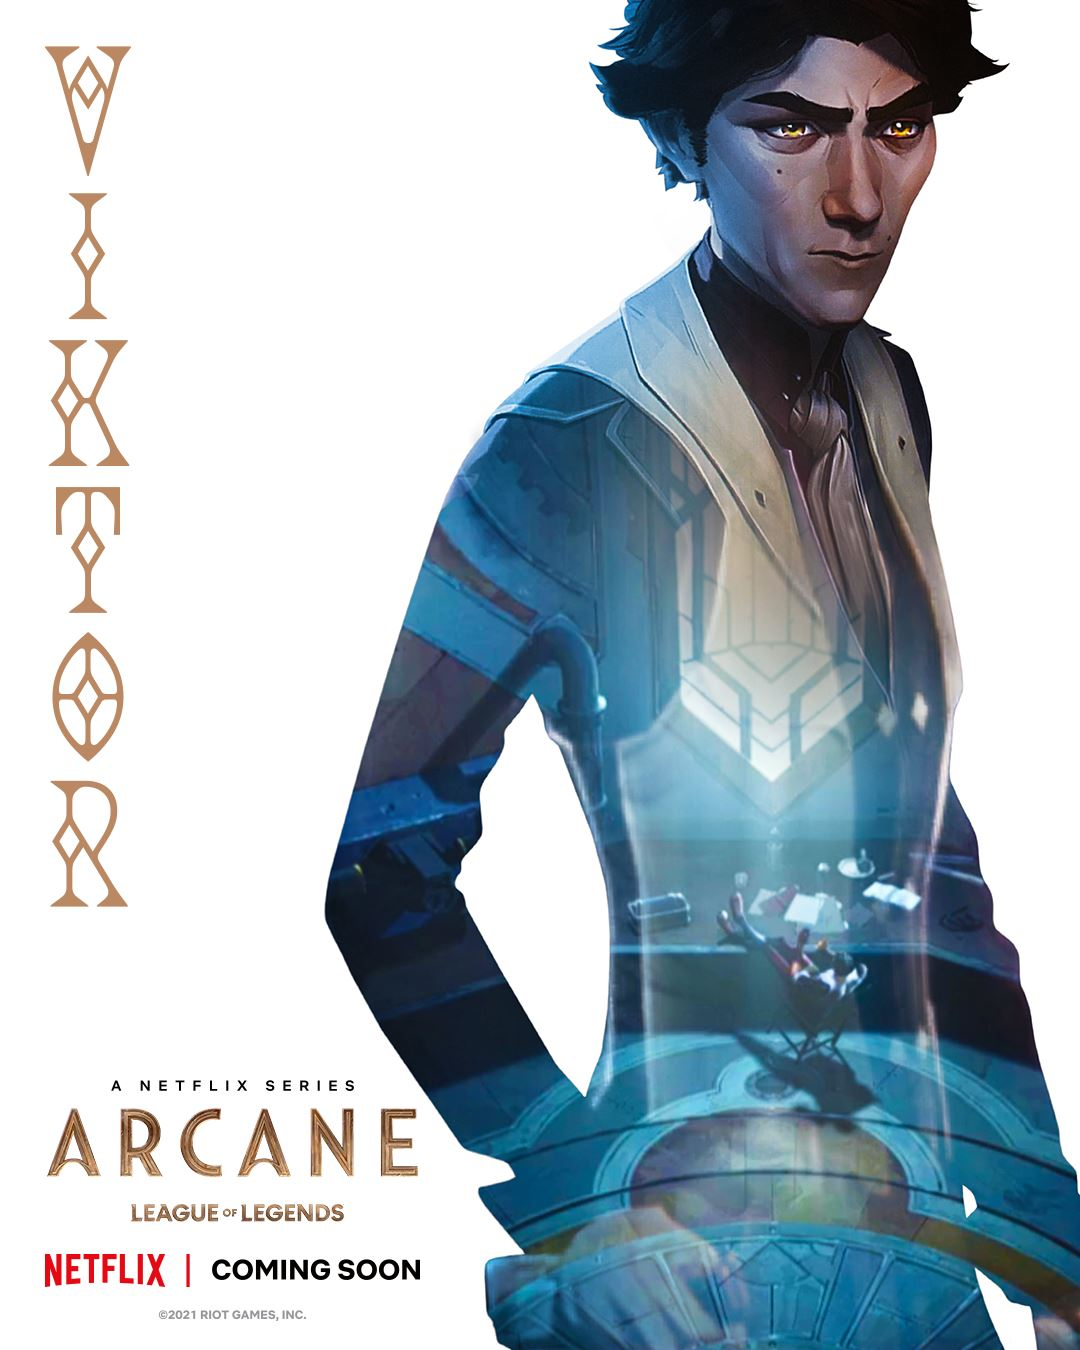
\includegraphics[scale=0.1, angle=18]{Pelicula. Imagenes usadas/Viktor, personaje favorito junto a otro.jpg}
    \caption{\textcolor{white}{Como un genio nato que nacio entre la pobreza, su papel pasado fue escapar de ahí y llegar a la grandeza, sin embargo, al lograrlo, su vida se acaba poco a poco debido a residuos de su pasado, por lo que ahora lucha por sobrevivir, a expensas de perder todo}}
    \label{fig:my_label}
\end{SCfigure}

\begin{SCfigure}
    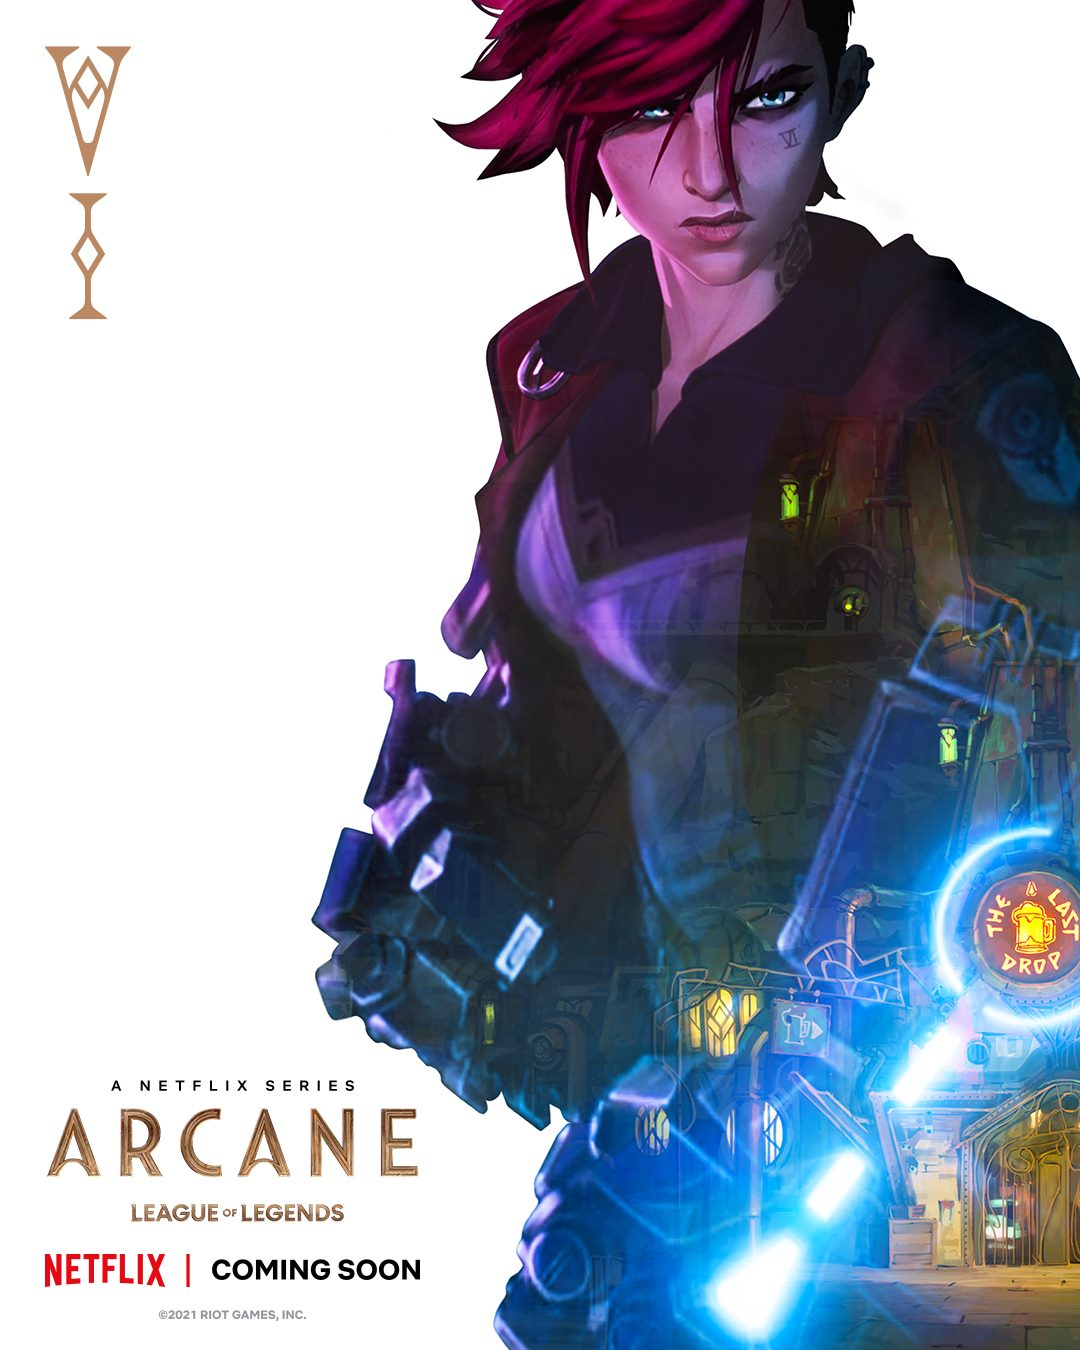
\includegraphics[scale=0.1, angle=-8]{Pelicula. Imagenes usadas/Vi, personaje menos favorito, pero que aún así es chido.jpg}
    \caption{\textcolor{white}{Perdió a todos los que amaba, pero incluso en esa situación mantiene su corazón y actitud firme, además que encuentra una nueva persona que proteger con su picante y pasional actitud}}
    \label{fig:my_label}
\end{SCfigure}

\hspace{-2.8cm}\textit{Si vas a}\newline
\vspace{-0.1cm}
\hspace{-2.9cm}\textit{cambiar el mundo,}\newline
\vspace{-0.1cm}
\hspace{-2.9cm}\textit{no pidas permiso.}\newline

\end{document}